\chapter{Literature Review}

\section{The Container Loading Problem}
\label{sec:clp_definition}

The placement and assignment of items to larger, mostly rectangular
containers, is a well known problem in logistics and operations research, as the
potential of cost savings and efficiency gains is substantial by reducing the number
of needed containers or by fulfilling customer needs. The \gls{CLP} covers a broad range of real-world applications,
such as loading cargo, optimizing warehouse storage and packing of pallets or cardboard boxes.
Generally it is differentiated in \textit{input minimization},
where the number of needed containers is minimized, and \textit{output maximization} problems,
where the value of the associated items is maximized. The \gls{BPP} is the generalized problem type of the \gls{CLP}
and belongs to \textit{input minimization} problems, whereas the knapsack problem to \textit{output maximization}. Apart from the expected outcome of the optimization,
the characterics of the items and containers is crucial for the problem definition. Items can be either
homogeneous or heterogeneous in size and shape. Furthermore, they can be classified as weakly or strongly
homogeneous or heterogeneous, depending on the degree of similarity among them. The container is
defined as a recangular volume with a fixed size and shape, where the items have to be placed in.
Other, non rectangular, shapes are seldomly considered in the literature, as the practical relevance is
limited. Multiple containers of homogeneous or heterogeneous sizes are used when the volume and weight
of the cargo require it.\footcite[cf.][pp. 1--2]{bortfeldt_constraints_2013}
According to \textcite{bischoff_issues_1995}, the mere placement of items in containers is insufficient
if practical requirements are not fulfilled as it lacks applicability. \footcite[cf.][pp. 1--2]{bischoff_issues_1995}
\textcite{bortfeldt_constraints_2013} systematically categorized all constraints emphasized in \gls{CLP} research
into five categories, which are presented in the following. They also distinguish between hard and soft constraints,
where hard constraints must be strictly satisfied, while soft constraints may be violated
to some extent.\footcite[cf.][p. 2]{bortfeldt_constraints_2013}  Figure~\ref{fig:solution-visualization}
visualizes a possible 3D packing with different constraints applied.

\begin{figure}[ht]
    \centering
    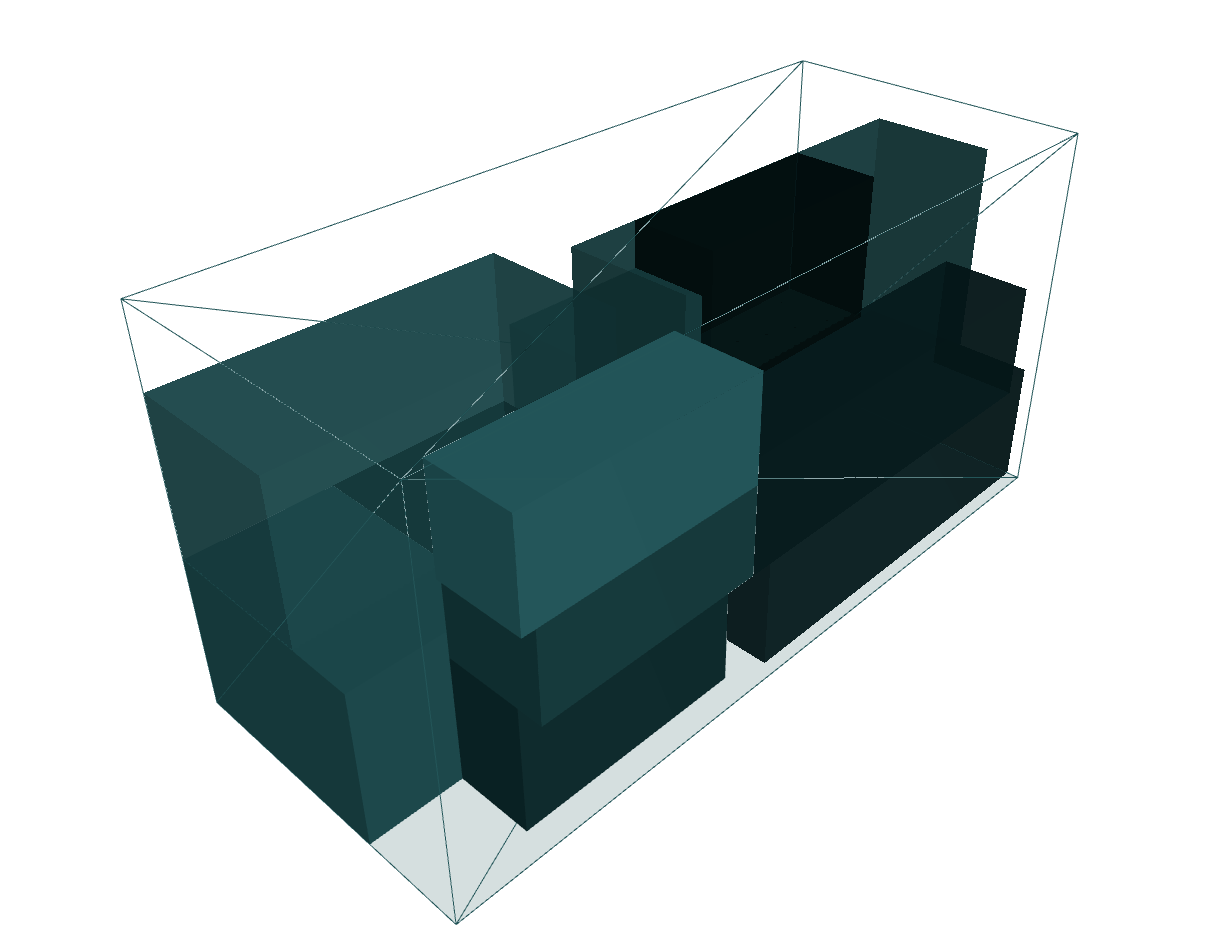
\includegraphics[width=6.3cm]{pictures/3l_cvrp_example.png}
    \caption[Visualized 3D packing with packing constraints.]{3D Packing with geometry, orthogonality and support area constraints.\footnotemark}.
    \footnotetext{CLP Visualizer from \textcite{tamke_branch-and-cut_2024}.}
    \label{fig:solution-visualization}
\end{figure}

\subsubsection{Container related constraints}
These constraints summarize all physical barriers of the container. The \textit{load capacity} limits the aggregated
mass of all items in the container. The distribution of the weight (\textit{load balance})
plays an important role for safety reasons, as the cargo must not move during the transport and the container
must not tip over and is defined by the maximum weight difference between the left and right half of the container.
When the containers are transported by trucks, uneven \textit{axle weight} distribution can cause severe
consequences and need to be avoided for practicability by loading the cargo axle-friendly. \footcite[cf.][pp. 849--850]{krebs_advanced_2021}

\subsubsection{Item related constraints}
Item related constraints define the properties of the item, which are relevant
for the packing. When the container capacity is limited (output maximization),
the \textit{loading priority} constraint defines the priority among possible
item candidates. The \textit{orientation} constraint restricts how an item can be rotated.
There are several types of rotation, each defined by the axis around which the item rotates.
The most common is the \textit{z-rotation}, where rotation is only allowed around the vertical axis.
When 3D packing is considered, stacking of items is allowed in comparison to 2D packing, when all
items are placed on the container floor. Two main approaches exist, when stacking is considered.
The \textit{fragility} constraint differentiates between fragile and non-fragile items,
allowing only non-fragile items to be stacked on non-fragile items. Figure \ref{fig:stacking_comparison} showcases
this definition. The other approach defines an individual \textit{\gls{LBS}} for each
item stating how much pressure the box can tolerate, and which items can be stacked. \footcite[cf.][pp. 847--848]{krebs_advanced_2021}

\begin{figure}[htbp]
    \centering
    \small
    % First TikZ picture
    \begin{subfigure}[b]{0.45\textwidth}
        \centering
        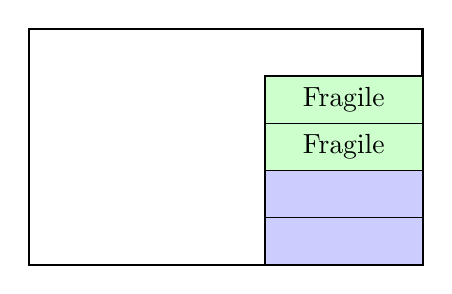
\begin{tikzpicture}
            % Draw the container
            \draw[thick] (0,0) rectangle (5,3);

            % Draw the three items inside
            \draw[fill=blue!20] (3,0) rectangle (5,0.6);
            \node at (4, 0.3) {};

            \draw[fill=blue!20] (3,0.6) rectangle (5,1.2);
            \node at (4, 0.9) {};

            \draw[fill=green!20] (3,1.2) rectangle (5, 1.8);
            \node at (4, 1.5) {Fragile};

            \draw[fill=green!20] (3,1.8) rectangle (5, 2.4);
            \node at (4, 2.1) {Fragile};

        \end{tikzpicture}
        \caption{Feasible stacking of items.}
    \end{subfigure}
    \hfill
    % Second TikZ picture
    \begin{subfigure}[b]{0.45\textwidth}
        \centering
        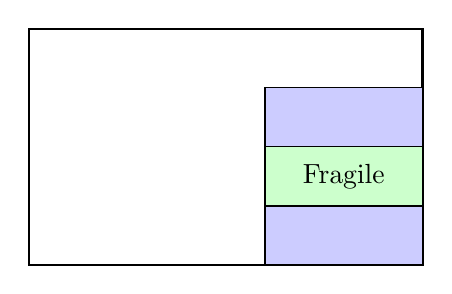
\begin{tikzpicture}
            \draw[thick] (0,0) rectangle (5,3);

            % Draw the three items inside
            \draw[fill=blue!20] (3,0) rectangle (5,0.75);
            \node at (4, 0.5) {};

            \draw[fill=green!20] (3,0.75) rectangle (5,1.5);
            \node at (4, 1.125) {Fragile};

            \draw[fill=blue!20] (3,1.5) rectangle (5, 2.25);
            \node at (4, 1.875) {};
        \end{tikzpicture}
        \caption{Infeasible stacking of items.}
    \end{subfigure}
    \caption[Visualization of fragility constraint.]{Comparison of fragile stacking (side view).}
    \label{fig:stacking_comparison}
\end{figure}


\subsubsection{Cargo-Related Constraints}
In contrast to item-related constraints, cargo-related constraints apply to
the entire cargo or to specific subsets of it. The \textit{complete-shipment} constraint
requires that all items within a shipment must either be loaded into the same
container or be left behind entirely. This constraint is important
when container capacity is limited (output maximization) and items
cannot be split. The \textit{allocation} constraint serves a similar purpose,
including the \textit{connectivity} constraint, which mandates that
certain items must be loaded into the same container, and the
\textit{separation} constraint, which requires specific items to
be distributed across different containers. For example, kitchen
shipments, comprising multiple packages, should be delivered together
to enable efficient installation. Conversely, items such as perfume and fresh
vegetables should be shipped separately due to incompatibility.

\subsubsection{Positioning constraints}

Positioning constraints determine, if items must be placed at
absolute locations or relative to other items. Absolute positioning is
typically based on item characteristics such as size, weight, or
content (e.g., bulky or hazardous items placed near the container door for accessibility) or
they may universally apply to all items, as the \textit{geometry} and
\textit{orthogonality} constraints. These constraints define that items are not allowed to overlap
and must be placed orhogonally to the container walls respectively.
Relative positioning requires items to be placed either close together as a \textit{group} or
\textit{separated} from each other.
The multi-drop constraint combines absolute and relative positioning requirements for items
destined for different delivery locations. The goal is to minimize reloading efforts by grouping items
by destination, arranging these groups in the delivery sequence, and applying either a \textit{\gls{LIFO}}
or sequential loading policy to ensure efficient unloading without having to move unrelated items.
Variations of the \gls{LIFO} constraint account for manual unloading (\textit{\gls{MLIFO}}) or unloading based on the
maximum allowable distance reachable from the unloading point (\textit{reachability}).

\subsubsection{Load-related constraints}

The \textit{stability} constraint is defined as one of the most critical constraints
in the \gls{CLP}, as it directly impacts the safety of both the cargo and the personnel involved.
First, a distinction must be made between \textit{horizontal} and \textit{vertical} stability.
Horizontal stability is achieved when items are securely connected to the
container walls or to other items, preventing lateral movement. Vertical
stability, on the other hand, is defined in various ways throughout the
literature. A common approach to assessing vertical stability is through the concept of the \textit{support
    area}, the portion of an item's base that rests on the surface below. Stability is typically
considered sufficient when the support area covers $75\%$ to $100\%$ of the item’s base. \footcite[cf.][p. 344]{gendreau_tabu_2006} However,
this may still result in unstable configurations if the center of gravity falls outside the
support area of the underlying layers, potentially causing the cargo to tilt. To improve practical stability,
a more reliable definition of vertical stability requires a minimum support area for all items below,
referred to as \textit{robust stability}.\footcite[cf.][p. 1140]{ceschia_local_2013} This comparison is illustrated in Figure~\ref{fig:vertical_stability_comparison}.
Additionally, it is crucial to ensure that the load remains stable even after partial unloading.
In addition, complexity constraints refer to specialized
requirements that are beyond standard packing rules. These include, for example, compatibility with automated or robot-assisted packing systems.

\begin{figure}[htbp]
    \centering
    \footnotesize
    % First TikZ picture
    \begin{subfigure}[b]{0.45\textwidth}
        \centering
        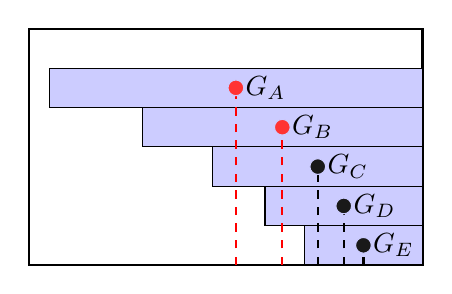
\begin{tikzpicture}
            % Draw the container
            \draw[thick] (0,0) rectangle (5,3);

            % Draw the three items inside
            % Draw the five items and their labels
            \draw[fill=blue!20] (3.5,0) rectangle (5,0.5);
            \draw[thick,dashed,black] (4.25,0) -- (4.25,0.25);  % <---
            \draw[fill = black!90, draw = blue!20] (4.25,0.25) circle (0.1);
            \node[anchor=west] at (4.25,0.25) {$G_E$};

            \draw[fill=blue!20] (3,0.5) rectangle (5,1);
            \draw[thick,dashed,black] (4,0) -- (4,0.75);  % <---
            \draw[fill = black!90, draw = blue!20] (4,0.75) circle (0.1);
            \node[anchor=west] at (4,0.75) {$G_D$};

            \draw[fill=blue!20] (2.33,1) rectangle (5,1.5);
            \draw[thick,dashed,black] (3.67,0) -- (3.67,1.25);  % <---
            \draw[fill = black!90, draw = blue!20] (3.67,1.25) circle (0.1);
            \node[anchor=west] at (3.67,1.25) {$G_C$};

            \draw[fill=blue!20] (1.44,1.5) rectangle (5,2);
            \draw[thick,dashed,red] (3.22,0) -- (3.22,1.75);  % <---
            \draw[fill=red!80, draw = blue!20] (3.22,1.75) circle (0.1);
            \node[anchor=west] at (3.22,1.75) {$G_B$};

            \draw[fill=blue!20] (0.26,2) rectangle (5,2.5);
            \draw[thick,dashed,red] (2.63,0) -- (2.63,2.25);  % <---
            \draw[fill=red!80, draw = blue!20] (2.63,2.25) circle (0.1);
            \node[anchor=west] at (2.63,2.25){$G_A$};


            %\node at (4, 1.875) {Fragile};
            %\node[anchor = west,align=center] at (2.9,2.5) {\small Center of \\  balance};

        \end{tikzpicture}
        \caption{Feasible, but unrobust, stacking with 75\% support area.}
    \end{subfigure}
    \hfill
    % Second TikZ picture
    \begin{subfigure}[b]{0.45\textwidth}
        \centering
        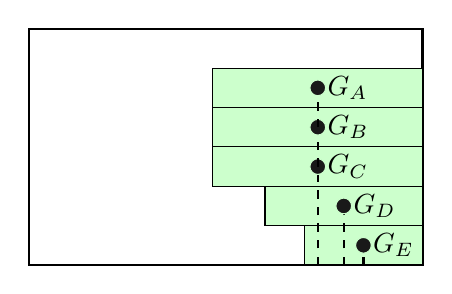
\begin{tikzpicture}
            % Draw the container
            \draw[thick] (0,0) rectangle (5,3);
            % Draw the three items inside
            % Draw the five items and their labels
            \draw[fill=green!20] (3.5,0) rectangle (5,0.5);
            \draw[thick,dashed,black] (4.25,0) -- (4.25,0.25);  % <---
            \draw[fill = black!90, draw = green!20] (4.25,0.25) circle (0.1);
            \node[anchor=west] at (4.25,0.25) {$G_E$};

            \draw[fill=green!20] (3,0.5) rectangle (5,1);
            \draw[thick,dashed,black] (4,0) -- (4,0.75);  % <---
            \draw[fill = black!90, draw = green!20] (4,0.75) circle (0.1);
            \node[anchor=west] at (4,0.75) {$G_D$};

            \draw[fill=green!20] (2.33,1) rectangle (5,1.5);
            \draw[thick,dashed,black] (3.67,0) -- (3.67,1.25);  % <---
            \draw[fill = black!90, draw = green!20] (3.67,1.25) circle (0.1);
            \node[anchor=west] at (3.67,1.25) {$G_C$};

            \draw[fill=green!20] (2.33,1.5) rectangle (5,2);
            \draw[thick,dashed,black] (3.67,1.25) -- (3.67,1.75);  % <---
            \draw[fill = black!90, draw = green!20] (3.67,1.75) circle (0.1);
            \node[anchor=west] at (3.67,1.75) {$G_B$};

            \draw[fill=green!20] (2.33,2) rectangle (5,2.5);
            \draw[thick,dashed,black] (3.67,1.75) -- (3.67,2.25);  % <---
            \draw[fill = black!90, draw = green!20] (3.67,2.25) circle (0.1);
            \node[anchor=west] at (3.67,2.25) {$G_A$};


            %\node at (4, 1.875) {Fragile};
            %\node[anchor = west,align=center] at (2.9,2.5) {\small Center of \\  balance};

        \end{tikzpicture}
        \caption{Feasible and robust stacking regarding 75\% support area.}
    \end{subfigure}
    \caption[Comparison of different vertical stability constraints.]{Comparison of different vertical stability constraints \\ with G = Center of Gravity (container side view). \footnotemark}
    \footnotetext{Own figures based on \textcite[p. 845]{krebs_advanced_2021}.}
    \label{fig:vertical_stability_comparison}
\end{figure}



\section{Classical Solution Approaches}
\label{sec:classical_solution_approaches}
The \gls{CLP} is a NP-hard combinatorial problem. \footcite[cf.][p. 11]{bortfeldt_constraints_2013}
Consequently, heuristics and metaheuristics were the dominating tools
in the early stages of this research field.\footcite[cf.][]{pisinger_heuristics_2002} The variety of methods
and their solution quality for solving the 2D \gls{CLP} developed in recent years. \footcite[cf.][p. 23]{iori_exact_2021}
The variety of 3D algorithms, especially for exact methods, is in comparison limited, as
\textcite{zhao_comparative_2016} elaborated in their survey. The following Figure~\ref{fig:solution_methods_overview}
presents this overview of the solution methods for the 3D \gls{CLP}.\footcite[cf.][]{zhao_comparative_2016}
It is divided in three categories constructive heuristics, metaheuristics
and exact methods. Hybrid methods and improvement heuristics are not explicitly shown in the figure,
as the former combines components from multiple categories, while the latter is subsumed within
metaheuristics. The depicted solution methods are described in the following.

\begin{figure}[htbp]
    \centering
    \resizebox{0.55\linewidth}{!}
    {
        \begin{tikzpicture}[grow cyclic, text width=2.7cm, align=flush center,
                level 1/.style={level distance=3.5cm,sibling angle=120},
                level 2/.style={level distance=3.5cm,sibling angle=50}
            ]

            \node {Solution Techniques \gls{CLP}}
            child { node {Metaheuristics}
                    child { node {Simulated Annealing}
                            child{node{One Stage Local Search Solver}}}
                    child { node {Tabu Search}}
                    child { node {Evolutionary Algorithm}}
                    child { node {Augmented extreme point-based heuristic}}
                }
            child { node {Exact \\ Methods}
                    child { node {Constraint Programming}}
                    child { node {Mixed-integer programming}}
                }
            child { node {Constructive Heuristics}
                    child { node {Layer/ Wall/ Tower Building}}
                    child { node {Corner Point Algorithms}
                            child{node{Minimize Waste Area}}}
                    child { node {Bottom-Left-Fill}
                            child{node{Deepest-Bottom-Left-Fill}}}
                    child { node {Maximum Touching Perimeter}
                            child{node{Maximum Touching Area}}}
                    child { node {Tree Search Algorithm}}
                }
            ;

        \end{tikzpicture}
    }
    \caption{Overview of solution methods for the container loading problem.}
    \label{fig:solution_methods_overview}
\end{figure}



\subsubsection{Constructive Heuristics}
For obtaining an initial feasible solution, two primary strategies are commonly
used depending on the heterogeneity of the items. In cases where the items are weakly homogeneous,
the problem dimensionality is reduced from 3D to 2D by constructing either
\textit{walls} or \textit{layers} of similarly sized items. These structures fill one
dimension of the container, typically either length and height or width and length, thereby
simplifying the remaining problem space. Moreover, when the layers or walls have
equal dimensions approximately, horizontal and vertical stability constraints are met.
Beyond these two dominant approaches, several adaptations exist to address item heterogeneity.
For example, \textcite{gehring_genetic_1997} propose the construction of item
\textit{towers}, in which boxes are stacked on top of other items so that the base of the box is covered completely
by the box below it.
This effectively reduces the dimensions from 3D to a 2D floor space arrangement,
similar to the \gls{PLP}. \footcite[cf.][pp. 402--406]{gehring_genetic_1997}
Another method involves forming \textit{blocks} composed of identically shaped items.
These blocks are treated as single entities
during packing, significantly reducing the number of elements to be handled and thus
lowering overall problem complexity.\footcite[cf.][p. 801]{liu_novel_2011} Even though constructive heuristics are quite simple,
they are still widely used because of their simplicity and efficiency to obtain fast solutions.
\footcite[cf.][pp. 11--13]{tamke_branch-and-cut_2024}

\subsubsection{Metaheuristics}
Once an initial solution is found, metaheuristics or improvement heuristics can be applied
to improve it. Therefore a solution representation, such as a permutation of items, is required
to conduct changes of the current solution. \gls{GA}s were
used to either improve the walls, towers or layers found by the constructive heuristics
or by improving the quality of the permutation of all items. \footcite[cf.][]{gehring_genetic_1997}
\gls{TS} is a widely used approach for \gls{BPP} and \gls{CLP}. It is based on
the idea of iteratively improving a solution by exploring its neighborhood and simultaneously
storing certain moves or complete solutions in a tabu list to avoid back-cycling to
previous solutions, feasible or infeasible ones. \footcite[cf.][pp. 344--345]{gendreau_tabu_2006} \gls{SA} has rarely been used as a
standalone metaheuristic in the context of \gls{CLP}. Instead, it is often combined
with other approaches to leverage its cooling schedule, which allows the acceptance of
worse solutions at higher temperatures. This helps the algorithm to escape local optima
early in the search and gradually transition into a more focused intensification phase as
the temperature decreases. \gls{GRASP} has the advantage of controlling the selection of new
cuboid candidates along a spectrum between completely random and full greedy choices. \footcite[cf.][]{moura_grasp_2005}

\subsubsection{Exact Algorithms}
Retrieving optimal solutions for the \gls{CLP} is computationally challenging in comparison
to finding good solutions with heuristics. The main difficulty is to represent packing
patterns and the constraints introduced in Chapter~\ref{sec:clp_definition} in a mathematical way.
Two prominent methods exist for modeling the \gls{CLP}. The first one is \gls{MIP}, which can be
formulated in two primary ways. One approach defines each possible packing pattern as
a variable. \footcite[cf.][pp. 29--30]{zhu_prototype_2012} The second approach models
the placement of items using discrete coordinate variables. \footcite[cf.][pp. 4--8]{moura_integrated_2009}
Both formulations can benefit from enhancements such as branch-and-price or branch-and-cut
methods, which reduce the search space and improve solution time.
The second main method is \gls{CP}, which offers a flexible alternative for handling
complex constraints, where the focus is to find feasible solutions primarily and
not fulfilling an optimization criterion directly. \footcites[cf.][pp. 5--8]{kucuk_constraint_2022}[cf.][pp. 7--11]{tamke_branch-and-cut_2024} \textcite{iori_exact_2021} states, that
\gls{CP} improved the results of 2D \gls{CLP} problems significantly and is a promising
field of future research.\footcite[cf.][p. 23]{iori_exact_2021}

\parbreak

In general exact methods are not capable of solving large instances with practical relevance
in reasonable computation time. However, they can be used to understand the structure
of optimal solutions to provide lower bounds and guidance for the development of future
heuristics. \footcite[cf.][p. 2]{tamke_branch-and-cut_2024} A possible approach to improving
the performance of exact algorithms is the use of speed-ups, such as pretrained \gls{ML} models.
These models can substitute parts of the algorithm's computation time by predicting solution
feasibility or by quickly identifying good solutions, thereby reducing the need for exact instance
solving in iterative procedures, as will be further discussed in the next chapter.

\section{Motivation for Feasibility Prediction}
\label{sec:motivation_feasibility_prediction}
This section explores how \gls{ML} algorithms can enhance \gls{CLP} solution strategies,
highlighting both benefits and limitations. Two papers will be
analyzed, which use predictive methods to accelerate the computation time. Before that,
a short introduction to classifiers will be conducted. It is important to note that
several \gls{ML} approaches address the \textit{on-line} \gls{BPP}, where the optimal placement
of individual items, arriving sequentially, must be determined.\footcite[cf.][p. 1]{ali_-line_2022}
Since this work focuses on the \textit{off-line} \gls{BPP}, where a placement for all items is determined
simultaneously, on-line approaches are not further considered. The emphasis is placed primarily
on \gls{ML}-based classifiers. These are supervised \gls{ML} algorithms predicting the
value of a categorical or binary output column, called label, based on the
values of other columns, called features. Classifiers learn from a labeled dataset,
where the correct output values are known in advance, and then use this knowledge to
make predictions on new, unseen data. The accuracy can be evaluated afterwards by comparing
the predicted labels with the actual labels. \footcite[cf.][]{kotsiantis_supervised_2007}
An exemplary train dataset is shown in Table~\ref{tab:classifier_label_data}.

\begin{table}[ht]
    \small
    \centering
    \begin{tabular}{@{}cccccc@{}}
        \toprule
        \textbf{Instance} & \textbf{Feature 1} & \textbf{Feature 2} & \dots  & \textbf{Feature n} & \textbf{Label} \\
        \midrule
        1                 & xxx                & x                  & \dots  & xx                 & True           \\
        2                 & xxx                & x                  & \dots  & xx                 & False          \\
        3                 & xxx                & x                  & \dots  & xx                 & True           \\
        \vdots            & \vdots             & \vdots             & \vdots & \vdots             & \vdots         \\
        \bottomrule
    \end{tabular}
    \caption[Exemplary training dataset for a classifier with known labels.]{Exemplary training dataset for a classifier with known labels. \footnotemark}
    \footnotetext{Adapted table from \textcite[p. 249]{kotsiantis_supervised_2007}.}
    \label{tab:classifier_label_data}
\end{table}


A classifier can be implemented using various \gls{ML} models such as \gls{LR},
\gls{ANN}, support vector machine, or others. However, the most crucial aspect of any
\gls{ML} model is the selection of data, particularly the choice of features and
the size of the training set, since many models can be easily preselected from available
libraries and be compared performance wise. The model attempts to learn correlations between the provided features
and the corresponding labels. If the features are poorly chosen, the model may fail
to capture the underlying patterns in the data. Additionally, if the training set
is too small, the model might not generalize well, ultimately lacking the ability
to accurately predict unseen data. Furthermore, it needs to be noted, that available
\gls{ML} models are not by nature superior to other models, but can significantly outperform
other models on specific application problem \footcite[cf.][pp. 250, 264]{kotsiantis_supervised_2007}.


\subsection{Objectices for ML approaches}
To compare different models and \gls{ML} approaches idetnical objectives are needed. The most common
measures rely on the output of the confusion matrix, which sorts the output along
their true and predicted labels.

\begin{table}[ht]
    \centering
    \begin{tabular}{@{}lcc@{}}
        \toprule
                                 & \textbf{Predicted Positive} & \textbf{Predicted Negative} \\
        \midrule
        \textbf{Actual Positive} & True Positive (TP)          & False Negative (FN)         \\
        \textbf{Actual Negative} & False Positive (FP)         & True Negative (TN)          \\
        \bottomrule
    \end{tabular}
    \caption{Confusion matrix (binary classification).}
    \label{tab:confusion_matrix}
\end{table}
The output can be used to calculate the accurac and F1 scote of the classification, which
helps to interpret the outcomes and compare different model types.

\[
    \text{Accuracy}=\frac{TP+TN}{TP+TN+FP+FN}
    \qquad
    \text{F1}=\frac{2\,TP}{2\,TP+FP+FN}
\]


The usage of classifiers is promising to complement exisiting algorithms, as shown in the following.


\subsubsection{Feasibility Classifier of the \cgls{2L-CVRP}}
A practical application of the \gls{CLP} is the integration in the \gls{VRP}, where
a number of customers need to be served with a set of items by a fleet of vehicles that have
to start from a depot and return. The goal is to minimize the total distance driven
by the vehicles. When considering multidimensional items, the NP-hard problem itself,
increases in complexity, as every tour is representing a \gls{CLP} itself. \footcite[cf.][pp. 1--2]{tamke_branch-and-cut_2024}
\textcite{zhang_learning-based_2022} used a binary classifier to predict the feasibility of the
loading of single tours to reduce the overall computation time in their exact branch-and-price
algorithm. As many single tours need to be evaluated, the \gls{FFNN} model, a special type of \gls{ANN} models, reduced the need
to control the solutions only when they are discarded or accepted. The default approach would be to
determine feasibility by applying a exact feasibility checker, such as a \gls{CP} or \gls{MIP} model.
The classifier performed well and had an accuracy of at most $94.1\%$. However, some simplifications were made,
they allowed no stacking of items tackling the \cgls{2L-CVRP} and no further constraints,
as unloading sequence, rotation or stability (see Chapter~\ref{sec:clp_definition}) were considered.
The classifier was trained with a dataset of 50,000 tours obtained by the underlying column generation
algorithm containing 17 hand-crafted features capturing geometric
and spatial characteristics of the packing problem. These include the ratio of the total item area
to the container floor area, as well as the mean, standard deviation, minimum, and maximum of
the following four indicators:
\begin{itemize}
    \item[1.] The ratio of item width to item height.
    \item[2.] The ratio of item width to the container width.
    \item[3.] The ratio of item height to the container height.
    \item[4.] The ratio of each item’s area to the total container area.
\end{itemize}
The \gls{FFNN} model was trained in many epochs
using the \textit{Mini-Batch Gradient Descent Algorithm}. By integrating the classifier into the
exisiting branch-and-price algorithm, the CPU time was reduced by $54.12\%$ and the frequency of
calling the exact feasibility checker by $87.22\%$ on average. However, the objective values are not significantly
lower and the authors assume that the prediction accuracy does not influence the solution quality
to a high extent, as the objectve values obtained by the branch-and-price algorithm with a \gls{LR} classifier are similar. \footcite[cf.][pp. 4, 9--15]{zhang_learning-based_2022}

\subsubsection{Pallet Size Classifier for the \gls{PLP}}
Another use case for \gls{ML} in packing problems is presented by \textcite{aylak_application_2021},
who focus on selecting the optimal pallet size in the context of the \gls{PLP}. Here a number of fixed items
need to be placed on pallets with fixed weight, length and height dimensions, optimizing the volume utilization
generating subsequently stability and minimizing the number of pallets needed. Based on real-life data
three candidate pallet sizes were considered and the best packing pattern must be found for each packing
configuration defined by the number of boxes and their uniform size. Therefore, multiple packing heuristics were applied to
generate feasible packing patterns and identify the best-performing. These are used as labels for several
\gls{ML} models, which were trained to predict the optimal pallet size based on four input features: the box
dimensions \{x,y,z\} and the demand quantity. Compared to the purely heuristic approach, the classifier-based
determination achieved a volume utilization improvement of $6.7\%$ and significantly reduced computation time.
However, the study did not consider additional constraints such as weight limits, stacking rules, or stability.\footcite[cf.][pp. 12--14]{aylak_application_2021}

\parbreak

These two examples demonstrate that classifiers can be successfully integrated into existing \gls{CLP}
algorithms to reduce computation time and overall complexity, provided the classifier is well trained.
However, training such a model is often time-consuming, and the practicality of both training and
integrating a classifier must be carefully evaluated on a case-by-case basis.
In the two examples presented, the number of constraints was relatively small, allowing the classifier
to be trained with a limited set of features. When more complex constraints are introduced, such as
\gls{LIFO} unloading rules or item fragility, the construction of numerical features that accurately
represent these constraints becomes significantly more challenging.
Moreover, results achieved by simple classifiers often lack practical relevance, since real-world
scenarios, such as loading large containers or trucks, inevitably involve multiple constraints that
must be taken into account. \footcite[cf.][pp. 1--2]{bischoff_issues_1995} Therefore, the development of a classifier is not only demanding but also
requires careful consideration to ensure a favorable cost-benefit ratio.
A particularly promising and practically relevant application is the prediction of the feasibility of single tours for the
\gls{3L-CVRP} with constraints, an extension of the \gls{2L-CVRP} example discussed earlier. In the
\gls{3L-CVRP}, a large number of routes must be evaluated to identify those that minimize the total
distance traveled by all vehicles. While the packing of requested items does not need to satisfy
optimization criteria, it must still be feasible under the given \gls{CLP} constraints.\footcite[cf.][]{tamke_branch-and-cut_2024}
As discussed in Chapter~\ref{sec:classical_solution_approaches}, the verification of
packing feasibility for each individual route is computationally expensive.
Here, classifiers can significantly boost performance of existing exact algorithms by rapidly predicting the feasibility of the route. The
exact packing solution is then only computed for the final solution candidates or before an infeasible classified solution
is discarded to avoid incorrect eliminations, as presented above.
To facilitate this approach, a comparison of various published \gls{3L-CVRP} datasets will be conducted
to compare and identify the most appropriate dataset for training a binary feasibility classifier.